%%%%%%%%%%%%%%%%%%%%%%%%%%%%%%%%%%%%%%%%%%%%%%%%%%%%%%%%%%%
% --------------------------------------------------------
% Rho
% LaTeX Template
% Version 2.1.1 (01/09/2024)
%
% Authors: 
% Guillermo Jimenez (memo.notess1@gmail.com)
% Eduardo Gracidas (eduardo.gracidas29@gmail.com)
% 
% License:
% Creative Commons CC BY 4.0
% --------------------------------------------------------
%%%%%%%%%%%%%%%%%%%%%%%%%%%%%%%%%%%%%%%%%%%%%%%%%%%%%%%%%%%

\documentclass[9pt,a4paper,twoside]{rho-class/rho}
\usepackage[english]{babel}

%% Spanish babel recomendation
% \usepackage[spanish,es-nodecimaldot,es-noindentfirst]{babel}

\setbool{rho-abstract}{true} % Set false to hide the abstract
\setbool{corres-info}{true} % Set false to hide the corresponding author section

%----------------------------------------------------------
% TITLE
%----------------------------------------------------------

\journalname{Ecology and Evolution}
\title{Altitude-Driven Adaptive Divergence In The Color-Polymorphic Bush Cricket \textit{Isophya rizeensis}
}

%----------------------------------------------------------
% AUTHORS AND AFFILIATIONS
%----------------------------------------------------------

\author[1]{Ufuk Topalan}
\author[2]{Arda Cem Kuyucu}
\author[1]{Salwa Ahmed Farid}
\author[1]{Mariam Younes}
\author[2]{Selim Süalp Çağlar}
\author[1,$\star$]{İsmail K. Sağlam}

%----------------------------------------------------------

\affil[1]{Department of Molecular Biology and Genetics, Koç University, Istanbul, Türkiye}
\affil[2]{Department of Biology, Hacettepe University, Ankara, Türkiye}
\affil[$\star$]{corresponding author}

%----------------------------------------------------------
% DATES
%----------------------------------------------------------

\dates{This manuscript was compile on January 17, 2025}

%----------------------------------------------------------
% FOOTER INFORMATION
%----------------------------------------------------------

\leadauthor{Topalan et al. 2025}
\smalltitle{Altitude-Driven Adaptive Divergence}

%----------------------------------------------------------
% ARTICLE INFORMATION
%----------------------------------------------------------

\corres{İsmail K. Sağlam}
\email{iksaglam@ku.edu.tr}

%----------------------------------------------------------
% ABSTRACT
%----------------------------------------------------------

\begin{abstract}
    The accelerating impacts of global environmental and climatic change present significant threats to biodiversity, emphasizing the need to understand how natural populations adapt to environmental gradients. \textit{Isophya rizeensis}, a univoltine bush cricket endemic to Turkey's Fırtına Valley, offers a compelling model for studying local adaptation, owing to its striking altitudinal color polymorphism in males. Lower-altitude populations predominantly exhibit black morphs, while higher altitudes are characterized by pale-green individuals, a pattern suggesting adaptation to microclimatic conditions rather than classical thermal melanism. Using RAD-seq data from 71 individuals across 10 populations, we identified $92,048$ high-confidence polymorphic loci, including $1,113$ putatively adaptive loci. Genetic analyses revealed significant differentiation driven by altitude, with Mantel tests confirming isolation by distance and selection. Mid-altitude populations exhibited higher genetic diversity, while extreme-altitude populations showed reduced diversity and fixation of adaptive loci, highlighting the dual influence of gene flow and selection. Genome-wide association studies identified 42 loci significantly associated with altitude, supporting the role of disruptive selection in shaping genetic variation and maintaining polymorphism along the gradient. Discriminant analysis of principal components (DAPC) revealed strong genetic differentiation between color morphs, with three major loci contributing to this separation. These loci exhibited bimodal genotype distributions, indicating the existence of distinct genetic groups linked to color morphs and their altitudinal distribution. This study underscores how environmental pressures shape adaptive and neutral genetic variation, maintaining diversity despite high connectivity. Our findings highlight the interplay between gene flow, selection, and local adaptation, providing valuable insights into the mechanisms driving biodiversity in montane ecosystems and informing conservation strategies in the face of climate change.
\end{abstract}

%----------------------------------------------------------

\keywords{Disruptive selection, Genetic Discrimination, Genotype-Environment Association, RAD sequencing}

%----------------------------------------------------------

\begin{document}
	
    \maketitle
    \thispagestyle{firststyle}
    % \tableofcontents
    \linenumbers

%----------------------------------------------------------

\section{Introduction}

    Environmental gradients, such as altitudinal and latitudinal shifts, serve as powerful natural laboratories for studying the processes shaping genetic and phenotypic variation in populations (\cite{Wogan2018}; \cite{Kelly2019}). These gradients provide key insights into the interplay between environmental factors and genetic diversity, revealing the selective forces driving local adaptation (\cite{Muir2014}). By examining phenotypic and genetic variation along these gradients, researchers can identify traits and genetic loci associated with survival in varying environments, offering a deeper understanding of the evolutionary and adaptive basis of biodiversity (\cite{Merilä2014}; \cite{Waldvogel2020}).
    
    Altitudinal gradients are particularly valuable for exploring these dynamics due to their steep environmental transitions over short geographic distances (\cite{Chown2003}; \cite{Flatt2016}). These gradients impose diverse selective pressures, including temperature, humidity, and resource availability, which can shape genetic differentiation through mechanisms such as isolation by distance (IBD) and local adaptation (\cite{Sexton2014}; \cite{Stankowski2017}; \cite{Bradburd2019}). Notably, studies combining altitudinal clines with genotype-environment association analyses have identified genetic regions linked to climatic parameters, further advancing our understanding of spatially varying selection (\cite{Hancock2011}; \cite{Slatyer2014}; \cite{Pluess2016}). Clinal variation, which manifests as gradual changes in traits or allele frequencies across environmental gradients, is an effective lens for examining the genetic underpinnings of local adaptation and response of organisms to environmental change (\cite{Mayekar2022}; \cite{Tyrmi2020}; \cite{Soliani2020}).
    
    One particularly well-documented form of clinal variation is adaptive color polymorphism in invertebrates, which often correlates with temperature and habitat variation. Color morphs in insects, for example, can influence thermoregulation, camouflage, and ecological niche partitioning, conferring advantages such as broader resource use, greater stability, and resilience to environmental changes (\cite{Forsman2008}; \cite{Zeuss2014}; \cite{Kozlov2022}). Thermal melanism, where darker individuals warm faster in cold environments, exemplifies the intricate relationship between environmental conditions and phenotypic variation (\cite{Clusella-Trullas2020}). However, deviations from this pattern in many ectotherms suggest that additional ecological factors may also play a role (\cite{Karlsson2008}; \cite{Goodman2021}).
    
    Beyond thermoregulation, adaptive color polymorphism enables populations with alternative color morphs to occupy distinct ecological niches, facilitating expanded distribution capacity and higher resilience to local extinctions compared to less variable species (\cite{Forsman2008}; \cite{Wennersten2009}; \cite{Kozlov2022}). This highlights the evolutionary significance of geographic variation in coloration and the importance of understanding its genetic basis. Such insights not only guide conservation strategies by identifying populations at risk (\cite{Forsman2016}) but also deepen our understanding of how evolutionary and ecological processes drive population differentiation and speciation (\cite{McLean2014}).
    
    The bush cricket \textit{Isophya rizeensis} (\cite{SEVGILI2003}), endemic to the Pontic Mountains of Turkey (Figure $1$), represents a model organism for studying these processes. This species inhabits a sharp altitudinal gradient ($300$–$2,200$ meters) and exhibits striking dorsal color polymorphism in males, with darker individuals (found at lower altitudes) transitioning to paler morphs at higher elevations (\cite{Çağlar2014}) (Figure $1$). Interestingly, this pattern contradicts the thermal melanism hypothesis, which associates dark coloration with higher, cooler habitats (\cite{CLUSELLATRULLAS2007}). Ecological and physiological studies in \textit{I. rizeensis} suggest that darker morphs warm faster and reach higher body temperatures than their pale green counterparts, which may be disadvantageous in subalpine habitats where surface temperatures can exceed 40°C due to intense solar radiation (Kuyucu et al., 2016). In these environments, paler coloration could be an adaptation to avoid overheating, offering a survival advantage in sparsely vegetated, thermally variable conditions. Despite these observations, the genetic basis of color polymorphism and its relationship with altitude remains poorly understood. Moreover, whether this phenotypic divergence is accompanied by population-level genetic differentiation driven by selection or neutral processes is an open question.
    
    In this study, we integrated genome-wide sequencing with high-resolution population genetic analyses to investigate the interplay between environmental gradients, phenotypic variation, and genetic diversity in \textit{I. rizeensis}. Specifically, we aimed to: 
    
    \begin{enumerate}
    \item Characterize the population genetic structure and connectivity along the altitudinal gradient, focusing on isolation by distance.
    \item Quantify patterns of genetic diversity and differentiation at neutral and adaptive loci to compare the effects of drift vs adaptive processes.
    \item Detect loci that may contribute to local adaptation, particularly those associated with altitudinal variation.
    \item Identify loci contributing to genetic discrimination between pale and dark color morphs and test for associations between color polymorphism and altitude.
    \end{enumerate}
    
    By addressing these objectives, we contribute to a deeper understanding of how environmental gradients shape genetic and phenotypic variation in natural populations. Our findings provide valuable insights into the genetic basis of survival along altitudinal gradients and the maintenance of intraspecific polymorphism. Specifically, we emphasize the importance of both neutral and potentially adaptive genetic variation in shaping responses to environmental changes, offering a clearer picture of how these dynamics influence population persistence across heterogeneous landscapes.

\section{Materials and Methods}

    \subsection{Sample Collection and Sequencing}

       \textit{I. rizeensis} (Orthoptera: Tettigoniidae: Phaneropterinae: Barbitistini) is a univoltine color polymorphic bush cricket species endemic to the Fırtına Valley and its surroundings regions within the Pontic Mountains of the Eastern Black Sea, Türkiye (Figure $1$). Specimens for this study were collected between June and August 2006 from 11 locations along an altitudinal gradient ranging from $450$ to $2,300$ meters above sea level in the Fırtına Valley (Figure $1$) and categorized according to color as described in \cite{Çağlar2014}. DNA was extracted from the hind femura of individuals using \textsc{e.z.n.a.}® Insect DNA Kit (Omega Bio-Tek) according to the manufacturer’s protocol. Paired-end RAD libraries were constructed using the PstI restriction enzyme, following the protocol detailed in \cite{Ali2016}. Sequencing was conducted at an average depth of 10X on an Illumina HiSeq4000 at the UC Davis Genome Center core facilities. In total we generated RAD sequencing data from $75$ \textit{I. rizeensis} individuals along the Fırtına Valley, averaging $5-7$ individuals per location/altitude.
    
    \subsection{Alignment and filtering}

        Due to the absence of a reference genome for \textit{I. rizeensis} or in a closely related species, we generated a de novo RAD sequence reference library following the custom procedure given in \cite{SağlamMolEcol2016} (for details see supplementary materials). Raw reads from each individual were aligned to the this set of reference RAD-contigs using the \textsc{bwa-mem} algorithm (\cite{Li2010}; \cite{Li2013}). Resulting \textsc{sam} files were converted to coordinate-sorted \textsc{bam} files using \textsc{samtools} (\cite{Danecek2021}), and duplicate reads were marked with \textsc{Picard tools} (http://broadinstitute.github.io/picard). Paralog regions were identified using the \textsc{ngsParalog} (https://github.com/tplinderoth/ngsParalog) and removed from subsequent analysis.

    \subsection{SNP discovery and genotyping}

        Polymorphic sites were identified using \textsc{angsd}  (\cite{Korneliussen2014}) by calculating genotype likelihoods (\texttt{-GL $1$}), major and minor alleles (\texttt{-doMajorMinor $1$}), minor allele frequencies (\texttt{-doMaf $1$}), and generating \textsc{BCF/VCF} files (\texttt{-doBcf $1$}). Polymorphic sites were filtered to include only those with a minor allele frequency (MAF) of $0.05$ or higher (\texttt{-minMaf 0.05}). Additional filtering parameters included a minimum base quality score of $20$ (\texttt{-minQ $20$}), a minimum mapping quality of $10$ (\texttt{-minMapQ $10$}), and a posterior genotype probability threshold of $0.85$ (\texttt{-postCutoff $0.85$}). Only properly paired reads ( \texttt{-only\_proper\_pairs $1$}) were considered, and sites were retained only if the probability of them being polymorphic was statistically significant (\textit{P} < $10^{-12}$). Finally we filtered out any site that had an average per individual read depth under $6X$ and was not present in at least $50\%$ of individuals in each population.

    \subsection{Population Genetic Structure}

        Population genetic structure was assessed using Principal Component Analysis (PCA). First, a genetic covariance matrix was calculated between individuals in \textsc{PCAngsd} (\cite{Meisner2018}) based on genotype likelihoods. The covariance matrix was then subjected to eigenvalue decomposition in R (\cite{R2024}, version 4.2.0) to extract the principal component axes summarizing genetic variation and the first two principal components (PCs) were visualized in R.
       
        Admixture analyses were conducted with \textsc{NgsAdmix} (\cite{Skotte2013}) to estimate individual ancestry proportions based on genotype likelihoods. Analyses were performed for K values ranging from $2-5$, with $10$ independent runs for each K value to account for stochastic variation and avoid convergence to local optima. The most likely number of clusters was identified using the $\Delta{K}$ method of \cite{Evanno2005}, which calculates the rate of change in log-likelihood values across successive K values. Admixture proportions for each K value were visualized in R, while the spatial distribution of genetic clusters was mapped using \textsc{ArcGIS} Pro (https://resources.esri.ca/).

    \subsection{Genetic Differentiation and Isolation By Distance (IBD)}

        Genetic differentiation was assessed by calculating pairwise $F_{ST}$ values between populations. Genome-wide $F_{ST}$ estimates were derived using \textsc{Angsd}, beginning with the calculation of the joint site frequency spectrum (2D-SFS) for each population pair. Global weighted $F_{ST}$ values were then computed with the \texttt{realSFS} module (\cite{Nielsen2012}). To evaluate patterns of isolation by distance (IBD), a Mantel test was performed to assess the correlation between geographic and genetic distances. A Euclidean distance matrix between populations was generated using the \textsc{Geographic Distance Matrix Generator} v1.2.3 (\Cite{Ersts2024}) and served as the predictor variable, while the linearized pairwise $F_{ST}$ matrix [$F_{ST}$/(1 - $F_{ST}$)] was used as the response variable. IBD patterns were analyzed through Pearson and Spearman correlation Mantel tests with 999 permutations, implemented in R using the \texttt{vegan package} (\cite{Oksanen2001}; \cite{Mantel1967}).
 
    \subsection{Comparing Neutral and Adaptive Genetic Variation}

        To identify putatively adaptive loci, we used the \texttt{pcadapt} function in \texttt{PCAngsd} (\cite{Meisner2018}), which detects outliers based on population structure (\cite{Luu2017}). The analysis was conducted using the Mahalanobis distance statistic across principal components, with significance determined by a chi-square ($\chi^2$) distribution with $K$ degrees of freedom based on the number of significant PC axes after correcting for multiple testing. We identified one significant principal component ($K = 1$) based on Velicier’s minimum average partial (MAP) test (\cite{Shriner2011}). To mitigate inbreeding effects, SNPs deviating from Hardy-Weinberg equilibrium due to inbreeding were filtered using the \texttt{--inbreedSites} and \texttt{--inbreed} options in \texttt{PCAngsd}, yielding a final dataset of $82,976$ SNPs, resulting in a genome-wide significance threshold of $6.03 \times 10^{-7}$ ($\chi^2 = 24.903$, $df = 1$, $\alpha = 0.05$) for determining putatively adaptive loci.

        Genetic diversity was estimated separately for neutral and adaptive loci by computing pairwise nucleotide differences ($\theta_{\pi}$) based on the folded site frequency spectrum (SFS) since we did not have a suitable outgroup for determining ancestral states. Allele frequency likelihoods were first calculated in \texttt{ANGSD} (\texttt{-doSaf 1}), followed by maximum likelihood estimation of the SFS using \texttt{realSFS}. Genome-wide $\theta_{\pi}$ was obtained using the \texttt{thetaStat} module (\texttt{-do\_stat}) by averaging per-site values across all RAD loci.

        To assess genetic differentiation, pairwise $F_{ST}$ values were calculated, and isolation by distance was evaluated via Mantel tests, correlating geographic and genetic distances separately for neutral and adaptive loci.


    \subsection{Genetic Variation Associated with Altitude}
    
        To investigate genetic variation associated with altitude, a genome-wide association study (GWAS) was conducted using score statistics (\texttt{-doAsso $2$}) in \textsc{Angsd}. The score test applies a generalized linear model framework, with posterior genotype probabilities as the dependent variable and altitude (\texttt{-yQuant}) as the predictor variable, calculating likelihood scores for each SNP independently (\cite{Skotte2012}).

        Association mapping included the identification of polymorphic sites (\texttt{-SNP\_pval 1e-06}), inference of major and minor alleles (\texttt{-doMajorMinor $1$}), and estimation of allele frequencies (\texttt{-doMaf $1$}). Stringent filtering criteria were applied to exclude SNPs with a minor allele frequency below $5\%$ (\texttt{-minMaf $0.05$}) or fewer than ten observations per genotype class (homozygous major, heterozygous, and homozygous minor; \texttt{-minHigh $10$}). Likelihood ratio test (LRT) scores for each SNP were converted to \textit{P}-values, assuming a chi-square ($\chi^2$) distribution with one degree of freedom. A Bonferroni correction was applied to control for multiple testing.
        
        To examine allele frequency patterns at significantly associated sites, the frequency of the reference allele (defined as the minor allele across the entire dataset) was plotted against altitude. This analysis highlights altitude-driven genetic variation by illustrating changes in allele frequencies with elevation.

    \subsection{Genetic Discrimination of Color Morphs}
        To investigate genetic variation associated with color morphs, a Discriminant Analysis of Principal Components (DAPC) was performed using the R package \texttt{adegenet} (v2.1.1; \cite{Jombart2008}; \cite{Jombart2011}). Genotypes were called in \textsc{Angsd} (\texttt{-doGeno $4$}) and exported as \texttt{VCF/BCF} files (\texttt{-doBcf $1$}) using a uniform prior (\texttt{-doPost 2}) and a posterior probability cutoff of $85\%$ (\texttt{-postCutoff $0.85$}). The DAPC retained principal component axes explaining up to $80\%$ of the variance, with color morph (dark vs. pale) specified as the grouping variable.
        
        To identify SNPs contributing most strongly to discrimination between color morphs, variable contributions of SNPs to the linear discriminant functions were examined. These contributions were hierarchically clustered using the \texttt{Average} method in the \texttt{snpzip} function of \texttt{adegenet}, grouping loci into "outlier" and "non-outlier" categories.
        
        Genotypic variation at the identified outlier loci was further explored by categorizing individuals based on genotypes either as heterozygous, homozygous for the minor allele, or homozygous for the major allele. Genotype distributions were visualized as a heatmap generated with \texttt{ggplot2} (\cite{ggplot2}), illustrating differences in genotypic states between dark and pale morphs.

\section{Results}

    \subsection{Alignment statistics and SNP discovery}

        Using our de novo reference assembly strategy, we identified $224,187$ unique RAD-loci ranging from $250$ to $800$ bp, with an average length of $324$ bp. Raw read alignments to the de novo set of reference RAD-contigs achieved a mapping success rate of $73\%$ to $83\%$, averaging $77\%$, with a mean individual read depth of approximately $5-6X$. Detailed data on raw read counts, raw alignments, and alignments after removing PCR duplicates are provided in Supplementary Table S1. Based on alignment statistics, we excluded individuals with fewer than $1,000,000$ aligned reads after all filters, resulting in a final dataset of $71$ individuals from $11$ locations (Table 1). Across all collection sites, we identified $9,616$ polymorphic loci and $92,048$ high-confidence SNPs (\textit{P} < $10^{-12}$) with a minor allele frequency $>0.05$, a minimum per individual read dept of $6X$ and present in $\geq50\%$ of individuals per population.
        
\begin{table}[!h]
    \small
    \captionsetup[table]{labelsep=space, 
        justification=raggedright, singlelinecheck=off}
    \caption{Altitude, coordinates, color category and samples sizes of \textit{I. rizeensis} used in this study.}
    \label{tab:my-table}
    \scalebox{1.3}{
    \begin{tabular}{@{}lllll@{}}
    \toprule
    Altitude (m) & Latitude & Longitude & Color & N \\ \midrule
    450          & 40.9856  & 40.9646   & DARK  & 7 \\
    850          & 40.9406  & 40.9850   & DARK  & 6 \\
    900          & 40.9166  & 40.9456   & DARK  & 7 \\
    1000         & 40.9075  & 40.9479   & DARK  & 7 \\
    1100         & 40.8880  & 40.9297   & PALE  & 7 \\
    1200         & 40.8630  & 40.9342   & PALE  & 5 \\
    1300         & 40.8638  & 40.9501   & PALE  & 5 \\
    1900         & 40.8548  & 41.0125   & PALE  & 7 \\
    2000         & 40.7998  & 40.9217   & PALE  & 7 \\
    2100         & 40.7995  & 40.9588   & PALE  & 7 \\
    2300         & 40.7915  & 40.9574   & PALE  & 6 \\ \bottomrule
    \end{tabular}%
    }
\end{table}

    \subsection{Population Genetic Structure and Differentiation}

        Principal Component Analysis (PCA) identified two distinct genetic clusters along PC1, corresponding to individuals from lower (dark-colored) and higher (pale-colored) altitudes (Figure 2A). However, PC1 and PC2 accounted for only $3.82\%$ and $2.08\%$ of the total genetic variation, respectively, indicating limited overall genetic divergence. A transitional zone was observed along PC1, comprising individuals from intermediate altitudes (1100–1900 meters).
        
        Admixture analysis, consistent with the PCA, identified K=3 as the optimal number of clusters (Supplementary Figure S1). Low and high altitude populations showed minimal admixture, predominantly belonging to distinct genetic ancestries whereas mid-altitude populations (1100–1900 meters) formed a transition zone with mixed ancestry, corroborating PCA findings (Figure 2B). Along the altitudinal gradient, the proportion of low-altitude ancestry (black) decreased, while high-altitude ancestry (green) increased, reflecting a reciprocal relationship between genetic components and elevation (Figure 2B).

        Pairwise $F_{ST}$ comparisons revealed relatively low genetic differentiation along the altitudinal gradient and between populations (< $0.05$), indicating substantial genetic connectivity across the landscape (Supplementary Figure $S2$). Despite the overall low divergence a Mantel test revealed a significant relationship between linearized $F_{ST}$  [$F_{ST}/(1 - F_{ST})$] values and geographic distance for both Pearson (\textit{$r_p$} = $0.838$, \textit{P} = $0.001$) and Spearman (\textit{$r_s$} = $0.869$, \textit{P} = $0.001$) correlation tests, indicating a clear pattern of IBD (Figure 2C).

    \subsection{Comparing neutral and adaptive variation}

        \textsc{PCAdapt} identified $1,113$ putatively adaptive and $81,863$ neutral loci. Genome-wide mean genetic diversity ($\theta_\pi$) was generally high across the altitudinal gradient, ranging from $0.058$ to $0.065$ (Figure $3A$, Table $S2$). Mean genetic diversity values for neutral and adaptive loci were largely similar along the altitudinal gradient. However, we observed a slight increase in neutral genetic diversity relative to adaptive genetic diversity at mid-altitudes (excluding $1,000$ meters), with significant differences in mean $\theta_\pi$ between $900$ and $1,900$ meters (Figure 3A, Table S2).
    
        To compare genetic divergence, separate Mantel tests assessed correlations between geographic distance and linearized $F_{ST}$ [$F_{ST}$/(1 - $F_{ST}$) for adaptive and neutral loci. Genetic divergence increased with geographic distance for both categories, but the relationship was significantly steeper for adaptive loci (\textit{$r_p$} = $0.91$, \textit{$r_s$} = $0.91$, \textit{$P$} = $0.001$) compared to neutral loci (\textit{$r_p$} = $0.84$, \textit{$r_s$} = $0.87$, \textit{$P$} = $0.001$) (Figure 3B). These results indicate greater divergence and signs of allelic fixation in adaptive loci at altitudinal extremes compared to neutral loci, suggesting a stronger role for selection in driving genetic differentiation along the altitudinal gradient.

    \subsection{Association mapping of altitudinal variation}

        Genome-wide association studies using altitude as a quantitative variable was based upon $53,901$ SNPs that passed all filters leading to a genome wide significance of $9.276\times10^{-7}$ ($\alpha = 0.05$; LRT > $24.07$). Based on this threshold we identified 102 loci significantly associated with genetic variation along the altitudinal gradient (Table S3). Allele frequency changes at these loci revealed two distinct patterns: at some loci, the reference allele (defined as the minor allele in the full dataset) showed elevated frequencies in low-altitude populations, while at others, it was more frequent at high altitudes (Figure 4). These opposing patterns suggest that different loci may be under selection at the extremes of the gradient. Such divergent allele frequency shifts align with the action of disruptive selection, which may play a crucial role in shaping genetic variation and promoting local adaptation across the altitudinal gradient.

    \subsection{Genetic Discrimination between Color Morphs}

        Discriminant analysis of principal components (DAPC) based on dark and pale color morphs clearly separated individuals into two groups along the first discriminant function (DF1), with a high posterior assignment probability (0.97; Figure 5A). Pale individuals were perfectly classified (posterior success = 1.0), while $92.6\%$ of dark individuals were correctly assigned, with only two misclassified as pale.
   
        DF1 loadings identified three major-effect loci significantly contributing to genetic differentiation between color morphs (Figure 5B). Genotype analysis revealed two distinct blocks: pale individuals were nearly fixed for the major allele, while dark individuals were predominantly heterozygous (Figure 5C). Notably, these loci were also significantly associated with altitude (Table S3), reinforcing the connection between color polymorphism and altitudinal variation.

\section{Discussion}

    Global biodiversity is facing mounting threats due to climate change and habitat degradation, with species that have narrow ranges or specialized ecological requirements being especially vulnerable. (\cite{Segan2016}; \cite{Wang2024}; \cite{Harvey2020}). Understanding the genetic and phenotypic mechanisms that enable species to adapt to environmental changes is essential for predicting biodiversity outcomes and designing effective conservation strategies (\cite{Merilä2014}; \cite{Kelly2019}; \cite{Waldvogel2020}).
    
    Studying the genetic basis of variation along environmental gradients, such as altitude, provides valuable insights into the evolutionary processes driving differentiation and diversity, while also revealing the mechanisms that enable species to adapt to changing conditions (\cite{Wogan2018}; \cite{Kelly2019}). This study represents the first detailed analysis of the genetic basis of color polymorphism in \textit{I. rizeensis} along an altitudinal gradient. The findings highlight how altitude acts as a selective force, shaping genetic variation at loci associated with coloration and driving local adaptation and genetic differentiation. More broadly, this work provides valuable insights into the maintenance of adaptive polymorphism in response to changing environmental conditions, contributing to a deeper understanding of how selection shapes genetic diversity in natural populations."
    
    \subsection{Population Structure and Genetic Connectivity}

        Our findings revealed clear genetic structuring along the altitudinal gradient in \textit{I. rizeensis}, characterized by a distinct pattern of isolation-by-distance (IBD) and the presence of discrete genetic clusters at high and low altitudes, despite clear patterns of admixture along mid altitudes. Low pairwise FST values (<0.05) indicate substantial genetic connectivity across populations, suggesting that gene flow mitigates complete isolation. However, altitude-specific selective pressures appear to promote local divergence and adaptation at both ends of the gradient (\cite{Tigano2016}; \cite{Wang2014}).
        
        The association between genetic clusters and color morphs underscores the role of altitude in shaping differentiation. Black morphs dominate low-altitude populations, while pale morphs prevail at higher altitudes, indicating that color polymorphism may function as an adaptive trait influenced by altitude-specific selective pressures (\cite{AhnesjöForsman2006}; \cite{Sandoval1994}). In the transitional zone, gene flow reduces absolute genetic differentiation, yet selective forces likely maintain divergence in key traits such as color morphs. This mirrors findings in other montane species, where local adaptation reinforces genetic structure even in the presence of substantial migration (\cite{Orsini2013}; \cite{Sexton2014}).
        
        These results highlight the complex interplay between gene flow and selection in shaping the genetic architecture and connectivity of \textit{I. rizeensis} populations.

    \subsection{Contrasting Neutral and Adaptive Loci Reveal Genetic Signatures of Altitudinal Adaptation}
 
        Analyses of genetic variation in \textit{I. rizeensis} revealed distinct patterns between adaptive and neutral loci, shedding light on the interplay of gene flow, selection, and environmental gradients. Neutral loci exhibited relatively uniform diversity across populations, with only slight fluctuations along the altitudinal gradient. Notably, mid-altitude populations showed a slight increase in neutral genetic diversity relative to adaptive loci, potentially reflecting the mixing of alleles from high- and low-altitude populations, a well-documented phenomenon in transition zones where gene flow is high (\cite{Byars2009}; \cite{Polato2017}; \cite{Cortázar-Chinarro2017}).

        In contrast, adaptive loci exhibited stronger genetic differentiation along the altitudinal gradient, with significantly greater divergence at higher and lower elevations. The steeper slope of genetic divergence for adaptive loci compared to neutral loci suggests that selection may play an important role in shaping differentiation at environmental extremes (\cite{Raeymaekers2017}; \cite{Cortázar-Chinarro2017}). Genome-wide association analyses further identified 102 loci significantly associated with altitude, with allele frequency shifts at these loci displaying two distinct patterns: some alleles increased in frequency at high elevations, while others were more common at lower elevations. These opposing patterns suggest that distinct loci may be under selection at altitudinal extremes, raising the possibility that disruptive selection plays a role in maintaining genetic variation across the gradient (\cite{White2021}; \cite{Wadgymar2022}).

        The observed allele frequency shifts provide compelling evidence for local adaptation shaping genetic variation across ecological gradients, reinforcing findings from other taxa that show strong environmental selection acting on spatially structured populations (\cite{Tigano2016}; \cite{Zancolli2019}). Disruptive selection may be particularly important in structuring these populations by favoring different alleles at different altitudinal extremes, which can lead to distinct adaptive peaks in genetic variation (\cite{Berdahl2015}; \cite{Forester2016}). Additionally, the stronger correlation between genetic divergence and geographic distance for adaptive loci, compared to neutral loci, suggests that isolation by environment (IBE) is a more prominent driver of genetic differentiation than isolation by distance (IBD), a pattern consistent with observations in other species experiencing strong environmental selection (\cite{Jiang2019}; \cite{Wagutu2022}; \cite{Wakamiya2023}).

        Overall, these findings highlight the critical role of adaptive loci in shaping the evolutionary trajectory of \textit{I. rizeensis} in response to environmental variation, illustrating how selection promotes local adaptation along altitudinal gradients.

    \subsection{Genetic Discrimination between Color Morphs}
    
        Discriminant analysis of principal components (DAPC) revealed strong genetic differentiation between dark and pale morphs, with three loci significantly contributing to this separation. Pale morphs were nearly fixed for the major allele, while dark morphs were predominantly heterozygous, reflecting a bimodal genotype distribution indicative of selective pressures (\cite{Prince2017}; \cite{Thompson2019}; \cite{PereiraMartins2022}). This bimodal distribution suggests the maintenance of two discrete genetic classes corresponding to color morphs, likely driven by environmental selection. The overlap between loci identified in DAPC and those in association mapping with altitude further highlights their role in both altitude-driven adaptation and color differentiation. This pattern aligns with findings in other taxa, where color polymorphism reflects a balance between multiple agents of selection along environmental gradients (\cite{Mullen2008}; \cite{Villoutreix2023}).

        Although the specific pathways associated with these loci remain unknown, studies show that genetic mechanisms underlying color variation vary widely across species. For instance, in Drosophila, pigmentation is influenced by dopamine-related genes and interactions with melanin synthesis pathways (\cite{Wright1987}; \cite{Wittkopp2003}), while in species like ladybirds and grasshoppers, color variation arises from species-specific mechanisms with limited connections to known melanin pathways (\cite{MICHIE2010}; \cite{Bastide2016}). This diversity in genetic mechanisms suggests that color polymorphisms in \textit{I. rizeensis} might likewise be shaped by a complex interplay of ecological and evolutionary factors, and varying biological pathways.
\section{Conclusion}

    This study highlights the complex interaction between gene flow, selection, and local adaptation in shaping the genetic and phenotypic diversity of \textit{I. rizeensis}. The clear genetic and phenotypic differentiation along the altitudinal gradient underscores the critical role of adaptive processes in maintaining biodiversity in montane ecosystems.
    
    Future research should focus on functional genomics to identify the specific genes and biological pathways that maintain color polymorphism in this species. Additionally, identifying the ecological and environmental selective pressures driving both color variation and spatial patterns of diversity will be essential. A deeper understanding of these mechanisms is crucial for elucidating how organisms adapt to changing environments and will inform conservation strategies to mitigate the effects of environmental change and habitat disruption.

\section{Author Contributions}
UT conducted laboratory work and conducted all analysis with contributions from IKS. SAF and MY assisted in laboratory work. ACK, HG and SSC took part in field studies and helped conceptualize the study. IKS conceptualized the study and wrote the manuscript with input from UT.

\section{Acknowledgments}
This work was supported by the The Scientific and Technological Research Council of Türkiye (TÜBİTAK), grant number 122Z038 and Hacettepe University Scientific Research Center Project No. 03 02 601 012. We are greatly thankful to Dr. Mike Ryan Miller and Dr. Sean O'Rourke for conducting RAD library preparation and sequencing at UC Davis.  

\section{Ethics Statement}
All field collections were done with approval from the General Directorate of Nature Conservation and National Parks of Türkiye under field permits E-21264211-288.04-5057102 and xxxxx.

\section{Conflicts of Interest}
Authors declare no conflict of interest.

\section{Data Availability Statement}
Raw sequence data are available from the NCBI SRA: SRRXXXXX (BioProject PRJNAXXXX). Command lines, shell scripts, and R scripts for conducting all analyses outlined in the study can be found at https://github.com/UfukTopalan/AdaptiveGenomics\_Isophya.

\printbibliography
\clearpage\section{Figures}
\begin{figure}[h]
\centering
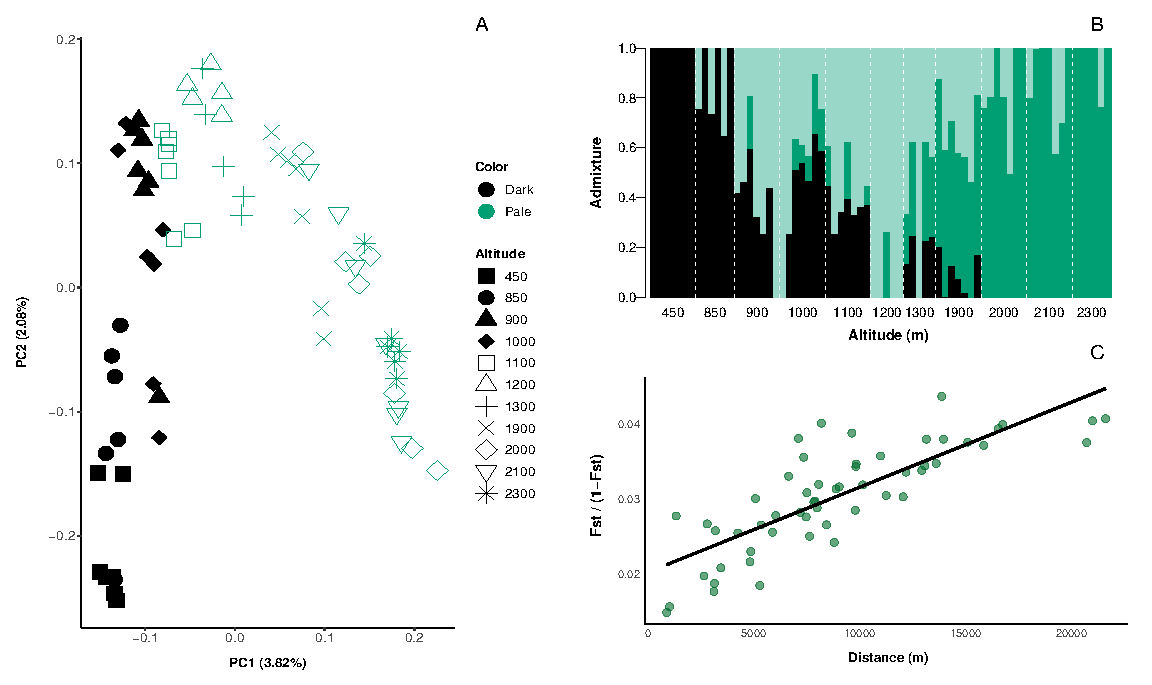
\includegraphics[width=1.8\columnwidth]{Figure_2.pdf}
\caption{Genetic structure and differentiation of \textit{I. rizeensis} along an alitudinal gradient in the Fırtına Valley. \textbf{(A)} Principal Component Analysis (PCA) of genetic variation, showing genetic structuring between lower-altitude (dark-colored) and higher-altitude (pale-colored) individuals along PC1. \textbf{(B)} Admixture proportions for $K=3$, illustrating distinct genetic ancestries at low (black) and high (green) altitudes, with mid-altitude populations exhibiting mixed ancestry. \textbf{(C)} Isolation-by-distance (IBD) pattern revealed by Mantel tests, showing significant patterns of genetic differentiation along the altitudinal gradient as measured by $F_{ST}$}
\label{Figure 2}
\end{figure}

\clearpage
\newpage
\begin{figure}[h!]
\centering
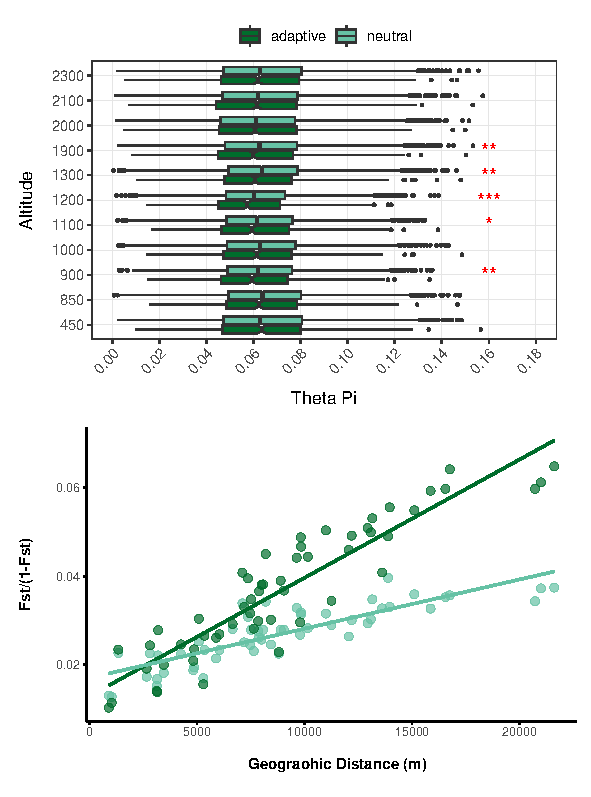
\includegraphics[width=0.8\columnwidth]{Figure_3.pdf}
\captionsetup[table]{labelsep=space, 
        justification=raggedright, singlelinecheck=off}
    \caption{Nucleotide diversity (A) and genetic differentiation (B) for adaptive and neutral loci in \textit{I. rizeensis} along an alitudinal gradient in the Fırtına Valley}
\label{Figure 3}
\end{figure}
\newpage
\begin{figure}[h!]
\centering
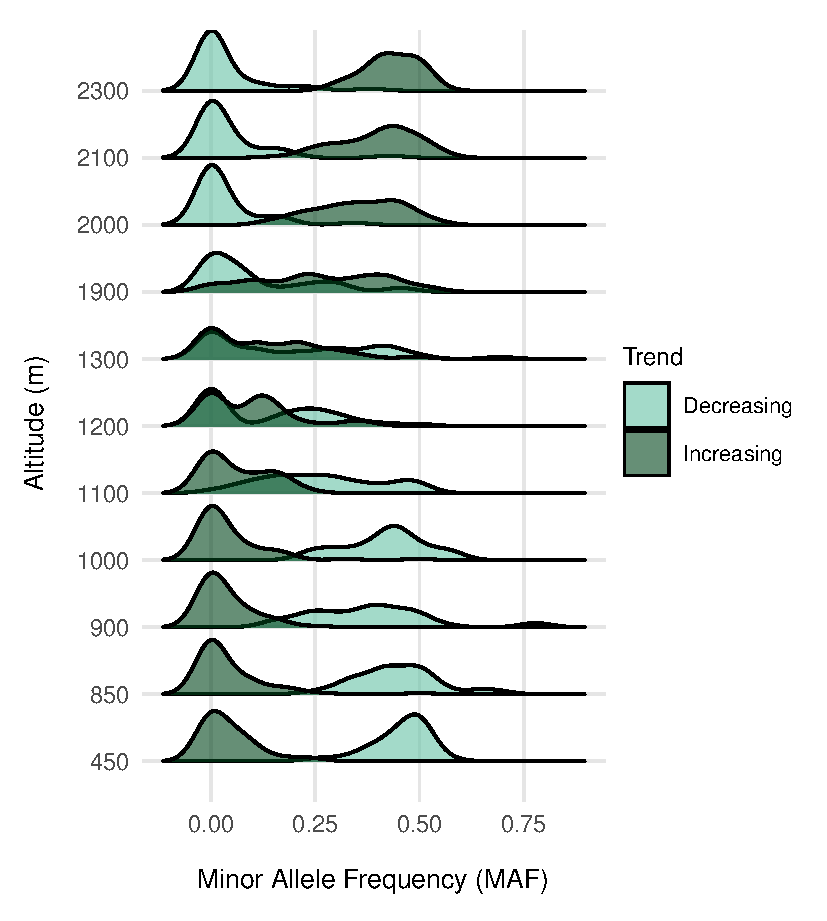
\includegraphics[width=0.8\columnwidth]{Figure_5.pdf}
\caption{Altitudinal variation in allele frequencies for the 102 SNPs significantly associated with elevation in \textit{I. rizeensis}, showing two distinct trends where the minor allele frequency either increases or decreases with altitude.}
\label{Figure 4}
\end{figure}

\begin{figure*}[b!]
\centering
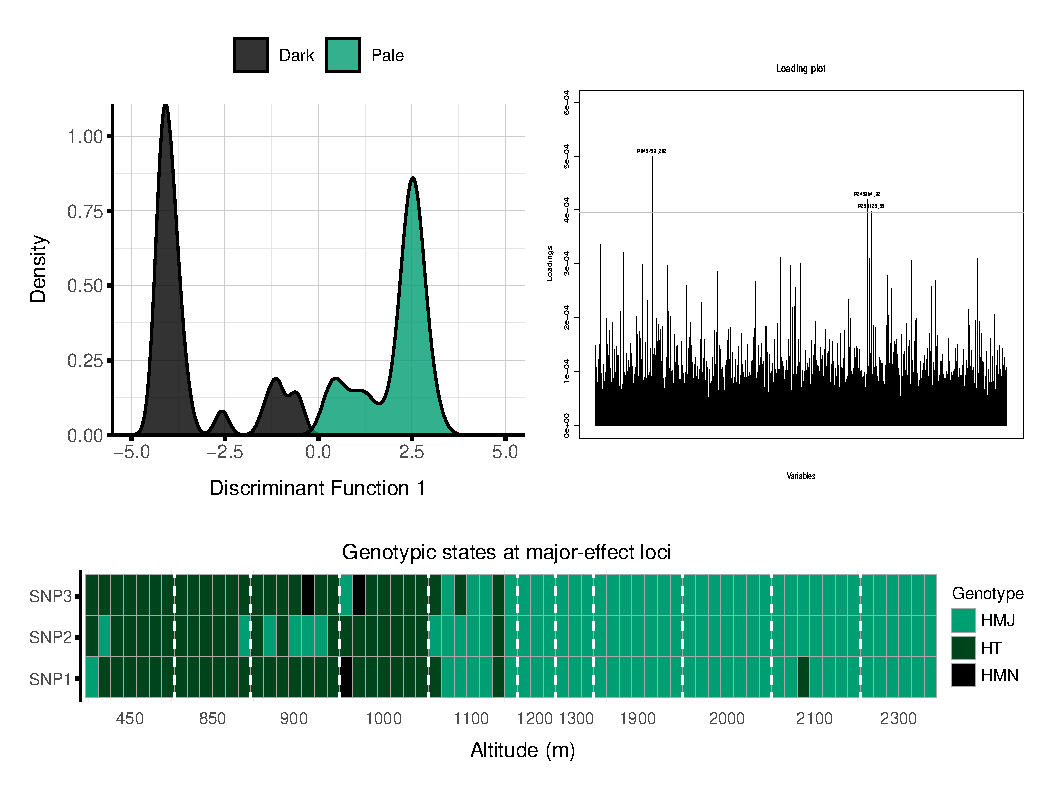
\includegraphics[width=1.8\columnwidth]{Figure_4.pdf}
\caption{Genetic differentiation between dark and pale color morphs of \textit{I. rizeensis} based on Discriminant Analysis of Principal Components (DAPC). (A) DAPC density plot along Discriminant Function 1 (DF1), showing clear separation between the morphs. (B) SNP loadings on DF1 identifying three major-effect loci contributing to morph differentiation. (C) Genotypic states at the three major loci along the altitudinal gradient.}
\label{Figure 5}
\end{figure*}

\end{document}